\section{Applying the Specification}\label{sec:standard}

\subsection{From patterns to clauses}

The 79 adopted forms were expressed as 106 numbered clauses, and every clause ends with a bracket that names the grounds it rests on.

Those brackets carry 183 links. Of them, 135 name an adopted form, 41 name one of the five principles, and 7 name a unit or a section of the goal document. A clause therefore stands on a mechanism, on a principle, or on the purpose I set for this work, and many stand on more than one.

The naming is structurally complete in both directions, and complete by computation rather than by assertion. Every one of the 106 clauses carries at least one link, at a mean of 1.73 and a maximum of 24. Every one of the 79 adopted forms is named by at least one clause, at a mean of 1.71 and a maximum of 6. Section~\ref{sec:results} reports the check that computes both.

The completeness is a property of the recorded grounding graph and nothing more. Every clause names grounds, and every adopted form is named by a clause. Whether a bracket names the right grounds is a separate question, settled by the clause-by-clause review of Section~\ref{sec:method} rather than by this count.

The clause carrying 24 grounds is the one that makes the minimum check set mandatory, and that spread is the point. A check set is where the rest of a normative document is enforced, so it inherits the grounds of everything it enforces.

One chain runs from a recorded practice to a check a reader can perform. The practice statement is that architecture decisions are kept as small numbered files beside the code they justify, under a fixed status vocabulary, and are never rewritten once accepted.

Generalization removed the software nouns and produced one adopted form. A binding decision is recorded as a numbered immutable record stating its context, the options considered with their trade-offs, the decision, its rationale, its consequences, and how compliance will be confirmed. Six other candidate statements were discarded into that one form.

Expression turned the form into four clauses on decision records and one on gate closure \citep[Sections~\hyperlink{nss-11.1}{11.1} to~\hyperlink{nss-11.4}{11.4} and~\hyperlink{nss-8.4}{8.4}]{pss2026}. The clauses fix what the record holds, the status vocabulary it draws from, the significance test that decides which decisions earn a record, and the rule that a reversal supersedes rather than edits.

The required record follows from the clauses: one decision record per binding decision, stored with the artifacts it governs. The check follows from the record: every record carries a status from the fixed vocabulary, and every supersession pointer resolves \citep[Section~\hyperlink{nss-16.2}{16.2}]{pss2026}.

What the chain buys is travel in both directions. A reader who doubts a clause reaches the practice statement it came from. A reader who changes an adopted form finds every clause that rests on it, which is the requirement of traversable consequence applied to this document.

External coverage of this family is one exploratory case study on the reuse of architecture decisions \citep{manteuffel2018}. That citation attributes a mechanism and validates no clause. No cited work supplied a clause.

Figure~\ref{fig:families} shows that the twelve mechanism families do not sit one to a section. Verification and acceptance reaches seven of the sixteen sections and contracts reaches six, because a rule about contracts constrains obligations, verification, baselines, and traceability alike. A reader who wants everything one family governs follows the brackets rather than the table of contents.

\begin{figure*}[t]
\centering
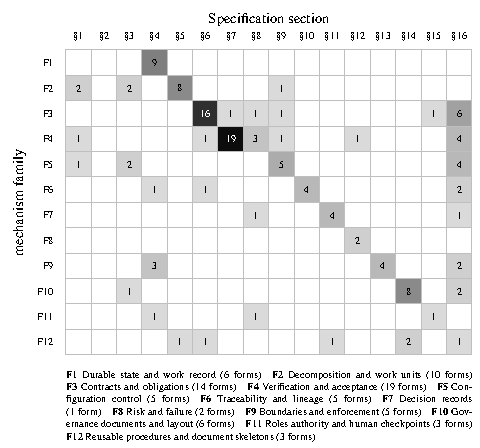
\includegraphics[width=\textwidth]{figures/f03/f03-family-section-matrix.pdf}
\caption{The twelve mechanism families against the sixteen sections of the Specification. A cell is marked where a clause of that section names a form of that family in its grounding bracket.}
\label{fig:families}
\end{figure*}

\subsection{Clause groups and their use}

The clauses fall into the twelve groups the twelve mechanism families produced: records, decomposition, contracts, verification, configuration, traceability, decisions, risk, executor limits, governance documents, authority, and procedures. Each group states a rule, requires a record or an action, and supports a check that reads what it required.

Records bind governing state to durable artifacts. Every state that governs work is a versioned artifact, with one canonical source per concern and any index over them generated rather than maintained by hand. The project record must be machine-readable. The check is blunt: an agreement that exists only in a session binds nothing. Provenance modelling supplies the shape such a record needs \citep{provdm2013}.

Decomposition binds work to units one executor can finish in one bounded effort. Each unit carries acceptance criteria and a declared blast radius, the set of elements it can affect \citep{kretsou2021}, and a unit whose blast radius cannot be bounded is split before it starts \citep[Section~\hyperlink{nss-5.6}{5.6}]{pss2026}.

Parallel units must have blast radii that do not overlap, because of what an overlap does to the estimate. Two units that can reach the same element bound nothing between them, since either can invalidate what the other was sized against. A defect in the shared element then belongs to no unit.

Two classes of unit are kept apart. A production unit changes the governed description under an approved plan. An exploratory unit runs in an isolated workspace with read-only access to the record, and nothing it produces governs anything. Work that proves out is redone as a production unit, and the exploratory record stays as evidence.

Contracts bind a component to what the rest of the system may rely on. Each component specification carries five sections a check can count: rationale, required behaviors, acceptance criteria, constraints, and dependencies and interfaces \citep[Section~\hyperlink{nss-6.2}{6.2}]{pss2026}. Each obligation is single, quantitative, and verifiable.

Each obligation also carries eight recorded attributes, among them a named human owner and the method that will verify it. An obligation missing one of them fails the check. Definition-of-done practice reports both the benefit of fixing completion that precisely and the difficulty of sustaining it \citep{kopczynska2022}.

Verification binds acceptance to text written before the work. The acceptance criterion and the verification method are authored with the obligation, and an obligation without a method does not enter an approved baseline. The executor that produced the work does not verify it.

Where one contract governs several realizations, one is designated the reference and compared with the others at a declared interval, so that divergence between what was specified and what was built is found on a schedule rather than at failure \citep{murphy2001}.

Configuration binds a description to a moment. Approved descriptions freeze as baselines, and one controlled gate governs every change to a locked one. A change re-issues the affected baseline entry and lands in the status ledger with an approving named human, a change class, and a marking of structural or behavioral \citep{iso15288}.

Traceability binds an obligation to the purpose above it and to the work below it. The links live in identifiers, naming, and placement, so any matrix over them is derived and never maintained by hand. The check refuses an obligation with no parent path to the vision document and one with no child path to realization elements and procedures. The backward direction is the one practitioners report as missing \citep{gotel1994}.

Decisions bind a choice to its reasons, and the chain above walks the group end to end. One rule reaches every other group: a decision record is the single home for the options considered and the rationale, and every other document points at it.

Risk binds an open exposure to a named closure. One register runs continuously, and a risk closes in exactly two ways, mitigated with evidence or accepted with a named human's rationale. The two are never recorded as one, because an accepted risk that reads as a mitigated one removes the grounds for revisiting it. Misuse and disuse of an automated control are documented failure modes, and a standing register is what keeps either one visible \citep{parasuraman1997}.

Executor limits bind an agent to a scope it cannot widen. Each executor's scope is declared once as a durable artifact, and its invariants are encoded as mechanical constraints rather than as prose, because a boundary that exists only as an instruction is a request \citep{saltzer1975}. Two rules follow: intermediate outputs are supervised for any attempt to weaken an acceptance criterion rather than meet it, and delegated work is isolated behind a condensed result.

Governance documents bind what an agent cannot discover from the system itself. One human-authored principles document states the reasoning the project applies, and every governance document stays under a declared size ceiling and references rather than copies. One study associates longer sessions with lower adherence \citep{mcmillan2026}, and the Specification therefore routes out of the document and into the versioned structure.

Authority binds every consequential judgment to a named human. One owner is named for the project, one for each component, and one for each obligation, and a standing function checks the work for flaws independently of whoever produced it. Seven authorities cannot be delegated: problem selection and purpose, invariants and safety boundaries, acceptance criteria and the definition of done, risk acceptance, resource and capital allocation, escalation decisions, and any commitment with external consequences, whether regulatory, financial, or contractual. AI agents may draft and propose in all seven and enact none of them.

Two consequences follow. The vision document and the governance documents are written and controlled by humans, because they carry purpose and reasoning rather than derived detail. The authority an action needs scales with its blast radius and with how hard it is to reverse \citep{parasuraman2000}.

Procedures bind recurring work to one definition. Work that recurs is written once as a reusable task definition: the steps in order, the acceptance criteria that close it, and the actions it forbids. Every design document spanning more than one work unit follows one skeleton and points at the decision records instead of restating them. The searched literature supplied no anchor for this group, which stands on the derivation record alone.

Four of the groups meet on one change. In the floating-city potable-water system of Section~\ref{sec:principles}, replacing a membrane module in the desalination train begins at the contract, in the obligation that fixes delivered water quality and names its owner and its verification method. Verification supplies the acceptance criterion and the procedure that tests it, and the agent that fitted the module does not run that procedure.

Traceability connects the work unit upward to the commitment made to the maritime authority and downward to the procedure that tests it, and the decision record holds why this membrane and not another. None of this requires reading the whole document. The reader finds the group, reads its clauses, and looks for the record the clauses name.

\begin{figure*}[!t]
\centering
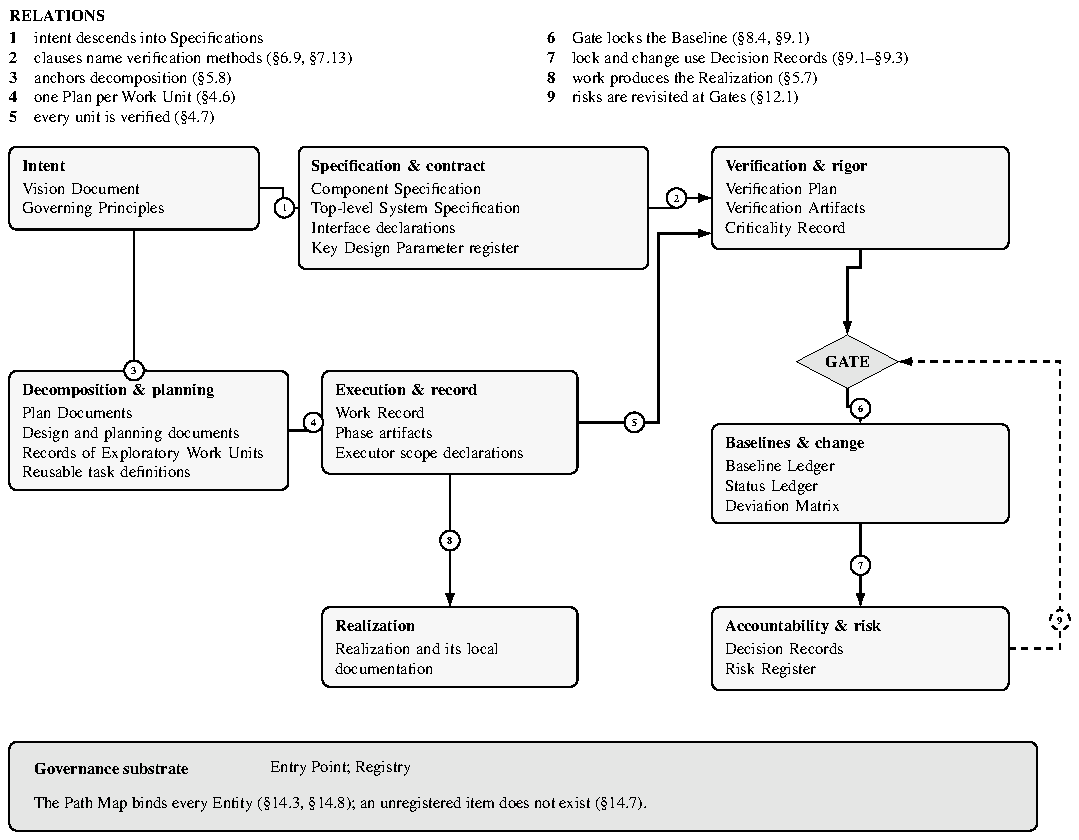
\includegraphics[width=\textwidth]{figures/f04/f04-entity-model.pdf}
\caption{The required Entities grouped by concern, with the relations the Specification declares between them. The governance substrate carries the Entry Point, whose Path Map binds every Entity to concrete storage, and the Registry, which holds the identity of every Component and content item. Drawn from the required Entity set of the Specification's \protect\hyperlink{nss-appA}{Appendix~A}.}
\label{fig:entities}
\end{figure*}

\subsection{Information model and reference binding}

A conforming project holds 24 required Entities, listed with their multiplicity in Table~\ref{tab:entities}. Figure~\ref{fig:entities} groups them by the concern each one serves and draws the relations between the groups. Intent reaches specifications, and specifications carry obligations that verification tests. Execution produces the record, baselines freeze what has been accepted, and decisions and risk attach to the baselines and the gates.

The model states which records must exist and how they refer to one another. It states nothing about where any of them lives, and the separation is deliberate \citep[Section~\hyperlink{nss-1.8}{1.8}]{pss2026}.

Four reasons hold it apart. A document that fixes file paths has confused its model with one storage of that model. Domains keep their records in their own formats, and a rule written for one format does not travel to another. Prose is the weakest artifact a check can read, so the binding has to name a format and not only a place. And a layout that serves one domain well is worth reusing rather than reinventing per project.

Each project declares a path map in its entry point that binds every required Entity to a location pattern and a serialization format. The binding is deterministic. An Entity with a multiplicity of one resolves to exactly one artifact, and for every artifact in the project record, its Entity is determinable from the map without judgement. The realization may sit outside the project record, wherever the map binds it, and the map declares its internal layout rather than classifying what is inside it. Checks resolve locations through the path map alone, so a check written once runs against a record laid out in any way the map can describe.

An Entity permitted zero instances is still bound. A project that runs no exploratory work unit binds that Entity to a pattern matching nothing, and the empty binding is what separates a project with no exploratory work from a project that lost the record of it.

One location is fixed, and it is the only one. The entry point is named \texttt{INDEX} and sits at the root of the project record, because a record whose map may be anywhere is not discoverable by anything that has not been told where to look.

Changing a locked description is not one act but a set of records, and which records depend on what changed. A change to a contract, an invariant, an acceptance criterion, or an artifact under human acceptance requires a new decision record. Every change to a locked baseline requires a status-ledger entry naming the re-issued snapshot, the approving human owner, the change class, and whether the change is structural or behavioral.

The affected baseline entry is then re-issued at the same locked status under the existing gate closure, and no new gate runs for a change that does not open one. Where the changed artifact is one the criticality record places under direct human acceptance, the change requires human authorization recorded in a decision record, and no automated procedure can supply it \citep[Sections~\hyperlink{nss-9.2}{9.2} and~\hyperlink{nss-7.19}{7.19}]{pss2026}.

Decision records are the one thing a change never edits. A superseded record keeps its text and gains a pointer from the record that replaced it, so the history stays readable in the order it happened.

The software profile offers one optional filesystem example. It uses Markdown for narrative records and JSON for structured records, with separate locations for specifications, plans, evidence, and registers. These choices illustrate how the required records can be stored; each project can select other locations and formats within the Specification.

A hardware profile gives a second optional example, for a physical system built from electronic, mechanical, and firmware components. The required records and their relations are the same as in the software example. What changes is the realization and its evidence. The built units are physical, so the example keeps their design and fabrication files in the formats of the design tools and describes each unit in an as-built record under its serial number. A bench measurement becomes a verification record that names the unit, the design release, and the instruments used. The domain changes the files and the evidence, while the required records and their relations stay the same. The example leaves domain-specific safety and regulatory practice to the methods and authorities of each domain.

A project that uses either example must complete its own path map and place every binding in its entry point. The local map must resolve without the external profile, including the locations and formats of the realization. Checks use that map and the declared format parsers, so changing storage preserves the required records and relations without making the example layout binding \citep[Section~\hyperlink{nss-14.8}{14.8}]{pss2026}.

\subsection{Scaled use and the minimum clause checks}

The smallest useful application is an ordered sequence and a short one. A vision document states the purpose. A criticality record fixes the class of the work and the reasoning for that class. An entry point declares the path map. One top-level specification carries the obligations, each with a named owner and a verification method. Decision records accumulate as binding choices are made, the ledgers and registers open empty, and the minimum checks run from the first day rather than from the first audit.

Every clause binds every project, and only depth scales. A two-person effort and a regulated capital programme both hold a contract, a verification method for each obligation, and a decision record for each binding choice. What the criticality class changes is how much evidence each one carries and how much independence its acceptance requires \citep[Sections~\hyperlink{nss-1.6}{1.6}, \hyperlink{nss-7.10}{7.10}, and~\hyperlink{nss-7.19}{7.19}]{pss2026}.

Scaling never reaches zero. An Entity is absent only through an entry in the deviation matrix naming what is waived, why, and which named human accepted the risk \citep[Section~\hyperlink{nss-1.5}{1.5}]{pss2026}. The matrix opens empty, so every absence in a conforming record is either declared or a defect.

A contained change shows the floor. Replacing the vendor of a chlorination setpoint controller in the floating-city water system touches one component, changes no obligation, and is recorded as a contained change in the status ledger against a re-issued baseline entry. No new gate runs and no acceptance is renewed, because the delivered water quality is unchanged and no commitment moved.

Shortening the 72-hour reserve is the same apparatus at a different depth. The reserve is an obligation the residents depend on and a commitment made to the maritime authority. The change therefore needs the authority to agree to a revised commitment, a decision record with the options and the accepted trade-offs, a re-issued contract, and a verification procedure that demonstrates the new figure. Acceptance is renewed by the named human owner, because a commitment with external consequences is not delegable \citep[Section~\hyperlink{nss-15.2}{15.2}]{pss2026}. Both changes use the same records. What differs is how many of them the change touches and how independent the acceptance has to be.

Sixteen checks are mandatory at minimum, and each one is written to detect a named class of defect. Six of them read the specification and its structure. They catch a specification missing one of its five sections, an unregistered component, and a registry entry that resolves to nothing. They catch an obligation without an owner or a verification method, and an obligation with no path upward to purpose or downward to work. They catch a circular dependency, a dependency on a less stable component, an acceptance criterion with no procedure, and a procedure with no clause.

The rest read the history and the substrate. They catch a decision record with an invalid status or a broken supersession pointer, a gate closed without a record, and a verification plan with no reference-realization designation or a designated contract with no comparison interval. They catch a baseline in an undeclared or dangling state, a locked baseline changed without a gate decision, and a change with no attribution or class. They catch a record with no discoverable entry point, a required Entity unbound or bound twice, and a governance document over its size ceiling. Table~\ref{tab:checks} states each check with the clause that imposes it and the defect class it detects.

A check that runs and leaves no trace does not count. The Specification states the rule as a flat sentence: ``A Normative Check whose outcome is not recorded has not run'' \citep[Section~\hyperlink{nss-16.3}{16.3}]{pss2026}. The outcome is itself a required record, which is what makes a result available to the next reader rather than only to whoever ran it.

The contract, configuration, and traceability records are what a change analysis reads. Section~\ref{sec:checks} states how a proposed edit is traced to everything it can affect, and that traversal runs over exactly these records.

Both requirements stated in the introduction are met by the same machinery. A clause carries its grounds, so a rule can be questioned without reconstructing why it exists. A record names what depends on it, so a change can be followed to its consequences before it is made. Section~\ref{sec:checks} turns the records into a representation a machine can traverse, and states what the traversal found.
